% Foliensatz: "AFu-Kurs nach DJ4UF" von DK0TU, Amateurfunkgruppe der TU Berlin
% Lizenz: CC BY-NC-SA 3.0 de (http://creativecommons.org/licenses/by-nc-sa/3.0/de/)
% Autoren: Sebastian Lange <dl7bst@dk0tu.de>
% Korrekturen: Lars Weiler <dc4lw@darc.de>

\documentclass[aspectratio=169]{beamer}

\usepackage[ngerman]{babel} % deutsche Worttrennung etc.
\usepackage[utf8]{inputenc} % UTF8 Text

\usepackage[super, comma, numbers, square, sort]{natbib}

\usepackage{hyperref}       % Hyperref Package für bessere Referenzen (todo)
\hypersetup{
	colorlinks=false,       %   false: boxed links; true: colored links
    %linkcolor=white,       %   color of internal links (change box color with linkbordercolor)
    citecolor=red,          %   color of links to bibliography
    filecolor=white,        %   color of file links
    urlcolor=blue           %   color of external links
}

\usepackage{multirow}
\usepackage{wasysym}  % Math Symbols like \permil
%\usepackage{colortbl}
%\usepackage{subscript}
%\usepackage{caption}
%\usepackage{setspace}
%\usepackage{xcolor}        % benutze CodeListe

% Footnote
%\usepackage{hanging}
%
%\setbeamertemplate{footnote}{%
%  \hangpara{2em}{1}%
%  \makebox[2em][l]{\insertfootnotemark}\footnotesize\insertfootnotetext\par%
%}


%\usepackage{pgf}
%\usepackage{tikz}
%\usetikzlibrary{arrows,automata}
%\usetikzlibrary{positioning}
%
%\tikzset{
%    state/.style={
%           rectangle,
%           rounded corners,
%           draw=black, very thick,
%           minimum height=2em,
%           minimum width=2pt,
%           inner sep=2pt,
%           text centered,
%           },
%}

%\usepackage{listings}
%\lstset{basicstyle=\small, numberstyle=\tiny, extendedchars=true, numbers=left, numbersep=5pt}
%\lstset{showtabs=false, showspaces=false, showstringspaces=false}
%%\lstset{backgroundcolor=\color{white!75!lightgray}, , frame=single}
%%\lstset{backgroundcolor=\color{white}}
%%\lstset{backgroundcolor=none}
%\lstset{keywordstyle=\color{blue!50!gray},  identifierstyle=\color{black}}
%\lstset{commentstyle=\color{green!50!gray}, stringstyle=\color{red!50!gray}}
%\lstset{language=C, fontadjust=true, tabsize=2, breaklines=true}
%\lstset{backgroundcolor=\color{white!75!lightgray}, caption=\lstname, frame=single}
%\lstset{emphstyle=\color{black}\fbox}
%
%% Keine "Listing:"-Caption
%\captionsetup{labelformat=empty,labelsep=none}
%
%% für mathematische Umgebungen
%\usepackage{amsmath,amsfonts,amssymb}
%
%\lstdefinestyle{Bash}{
%language=Bash,
%frame=single,
%rulecolor=\color{black},
%backgroundcolor=\color{gray!50},
%keywordstyle=\color{black},
%identifierstyle=,
%commentstyle=\color{black},
%stringstyle=\color{magenta!65!white},
%showstringspaces=false,
%basicstyle=\footnotesize\ttfamily\color{black},
%numbers=none,
%breaklines=true,
%captionpos=b
%}

%\usepackage{listings}
%
%\lstdefinestyle{basic}{
%    captionpos=t,%
%    basicstyle=\footnotesize\ttfamily,%
%    numberstyle=\tiny,%
%    numbers=left,%
%    stepnumber=1,%
%    frame=single,%
%    showspaces=false,%
%    showstringspaces=false,%
%    showtabs=false,%
%    %
%    keywordstyle=\color{blue},%
%    identifierstyle=,%
%    commentstyle=\color{gray},%
%    stringstyle=\color{magenta}%
%}



% fließende Boxen haben keinen Abstand
%\fboxsep0mm

% inkludiere Creative Commons Helper
%%%%%%%%%%%%%%%%%%%%%%%%%%%%%%%%%%%%%%%%%%%%%%%%%%%%%%%%%%%%%%%%
%% ccBeamer 0.1, 2007-07-02                                   %%
%% Written by Sebastian Pipping <webmaster@hartwork.org>      %%
%% ---------------------------------------------------------- %%
%% Licensed under Creative Commons Attribution-ShareAlike 3.0 %%
%% http://creativecommons.org/licenses/by-sa/3.0/             %%
%%%%%%%%%%%%%%%%%%%%%%%%%%%%%%%%%%%%%%%%%%%%%%%%%%%%%%%%%%%%%%%%


%% Images
\newcommand{\CcImageBy}[1]{%
	
\includegraphics[scale=#1]{texdata/creative_commons/cc_by_30.pdf}%
}
\newcommand{\CcImageCc}[1]{%
	
\includegraphics[scale=#1]{texdata/creative_commons/cc_cc_30.pdf}%
}
\newcommand{\CcImageDevNations}[1]{%
	
\includegraphics[scale=#1]{texdata/creative_commons/cc_dev_nations_30.pdf}%
}
\newcommand{\CcImageNc}[1]{%
	
\includegraphics[scale=#1]{texdata/creative_commons/cc_nc_30.pdf}%
}
\newcommand{\CcImageNd}[1]{%
	
\includegraphics[scale=#1]{texdata/creative_commons/cc_nd_30.pdf}%
}
\newcommand{\CcImagePd}[1]{%
	
\includegraphics[scale=#1]{texdata/creative_commons/cc_pd_30.pdf}%
}
\newcommand{\CcImageSa}[1]{%
	
\includegraphics[scale=#1]{texdata/creative_commons/cc_sa_30.pdf}%
}
\newcommand{\CcImageSampling}[1]{%
	
\includegraphics[scale=#1]{texdata/creative_commons/cc_sampling_30.pdf}%
}
\newcommand{\CcImageSamplingPlus}[1]{%
	
\includegraphics[scale=#1]{texdata/creative_commons/cc_sampling_plus_30.pdf}%
}


%% Groups
\newcommand{\CcGroupBy}[2]{% zoom, gap
	\CcImageCc{#1}\hspace*{#2}\CcImageBy{#1}%
}
\newcommand{\CcGroupByNc}[2]{% zoom, gap
	\CcImageCc{#1}\hspace*{#2}\CcImageBy{#1}\hspace*{#2}\CcImageNc{#1}%
}
\newcommand{\CcGroupByNcNd}[2]{% zoom, gap
	\CcImageCc{#1}\hspace*{#2}\CcImageBy{#1}\hspace*{#2}\CcImageNc{#1}\hspace*{#2}\CcImageNd{#1}%
}
\newcommand{\CcGroupByNcSa}[2]{% zoom, gap
	\CcImageCc{#1}\hspace*{#2}\CcImageBy{#1}\hspace*{#2}\CcImageNc{#1}\hspace*{#2}\CcImageSa{#1}%
}
\newcommand{\CcGroupByNd}[2]{% zoom, gap
	\CcImageCc{#1}\hspace*{#2}\CcImageBy{#1}\hspace*{#2}\CcImageNd{#1}%
}
\newcommand{\CcGroupBySa}[2]{% zoom, gap
	\CcImageCc{#1}\hspace*{#2}\CcImageBy{#1}\hspace*{#2}\CcImageSa{#1}%
}
\newcommand{\CcGroupDevNations}[2]{% zoom, gap
	\CcImageCc{#1}\hspace*{#2}\CcImageDevNations{#1}%
}
\newcommand{\CcGroupNcSampling}[2]{% zoom, gap
	\CcImageCc{#1}\hspace*{#2}\CcImageNc{#1}\hspace*{#2}\CcImageSampling{#1}%
}
\newcommand{\CcGroupPd}[1]{% zoom
	\CcImagePd{#1}%
}
\newcommand{\CcGroupSampling}[1]{% zoom
	\CcImageSampling{#1}%
}
\newcommand{\CcGroupSamplingPlus}[1]{% zoom
	\CcImageSamplingPlus{#1}%
}


%% Text
\newcommand{\CcLongnameBy}{Attribution}
\newcommand{\CcLongnameByNc}{Attribution-NonCommercial}
\newcommand{\CcLongnameByNcNd}{Attribution-NoDerivs}
\newcommand{\CcLongnameByNcSa}{Attribution-NonCommercial-ShareAlike}
\newcommand{\CcLongnameByNd}{Attribution-NoDerivs}
\newcommand{\CcLongnameBySa}{Attribution-ShareAlike}

\newcommand{\CcNote}[1]{% longname
	This work is licensed under the \textit{Creative Commons #1 3.0 License}.%
}


% generelles Thema auswählen
\usetheme{Goettingen} %Berlin spart ohne Sidebar allerdings angenehm Platz
% AnnArbor | Antibes | Bergen | Berkeley | Berlin | Boadilla | boxes | CambridgeUS | Copenhagen | Darmstadt | default | Dresden | Frankfurt | Goettingen | Hannover | Ilmenau | JuanLesPins | Luebeck | Madrid | Malmoe | Marburg | Montpellier | PaloAlto | Pittsburgh | Rochester | Singapore | Szeged | Warsaw

% Farben wählen
\usecolortheme{beetle}
% beaver | beetle | crane | default | dolphin | dove | fly | lily | orchid | rose | seagull | seahorse | sidebartab | structure | whale | wolverine

% Setze alle Farben auf Grau und Weiß
%\definecolor{craneorange}{RGB}{64,64,64}
%\definecolor{craneblue}{RGB}{255,255,255}

% Schriftart wählen
\usefonttheme{default}
% default | professionalfonts | serif | structurebold | structureitalicserif | structuresmallcapsserif

% Innere Themen(Kopf-, Fuß-, Sidebar usw)
%\useinnertheme{default}
\useinnertheme{circles}
% default | inmargin | rectangles | rounded | circles

% Äußere Themen (Anordnung der inneren, grenzen der Folien etc.)
\useoutertheme{infolines}
% default | infolines | miniframes | shadow | sidebar | smoothbars | smoothtree | split | tree

% Deaktiviere Navigations-Symbole ({} -> leer)
\setbeamertemplate{navigation symbols}{}
%\setbeamertemplate{navigation symbols}{\large \ifnum \insertframenumber <10 0\fi\insertframenumber/\inserttotalframenumber\vspace*{0.2ex}}

% Zeige ein Hintergrundbild
\setbeamertemplate{background canvas}{
        \hspace*{-2.0cm}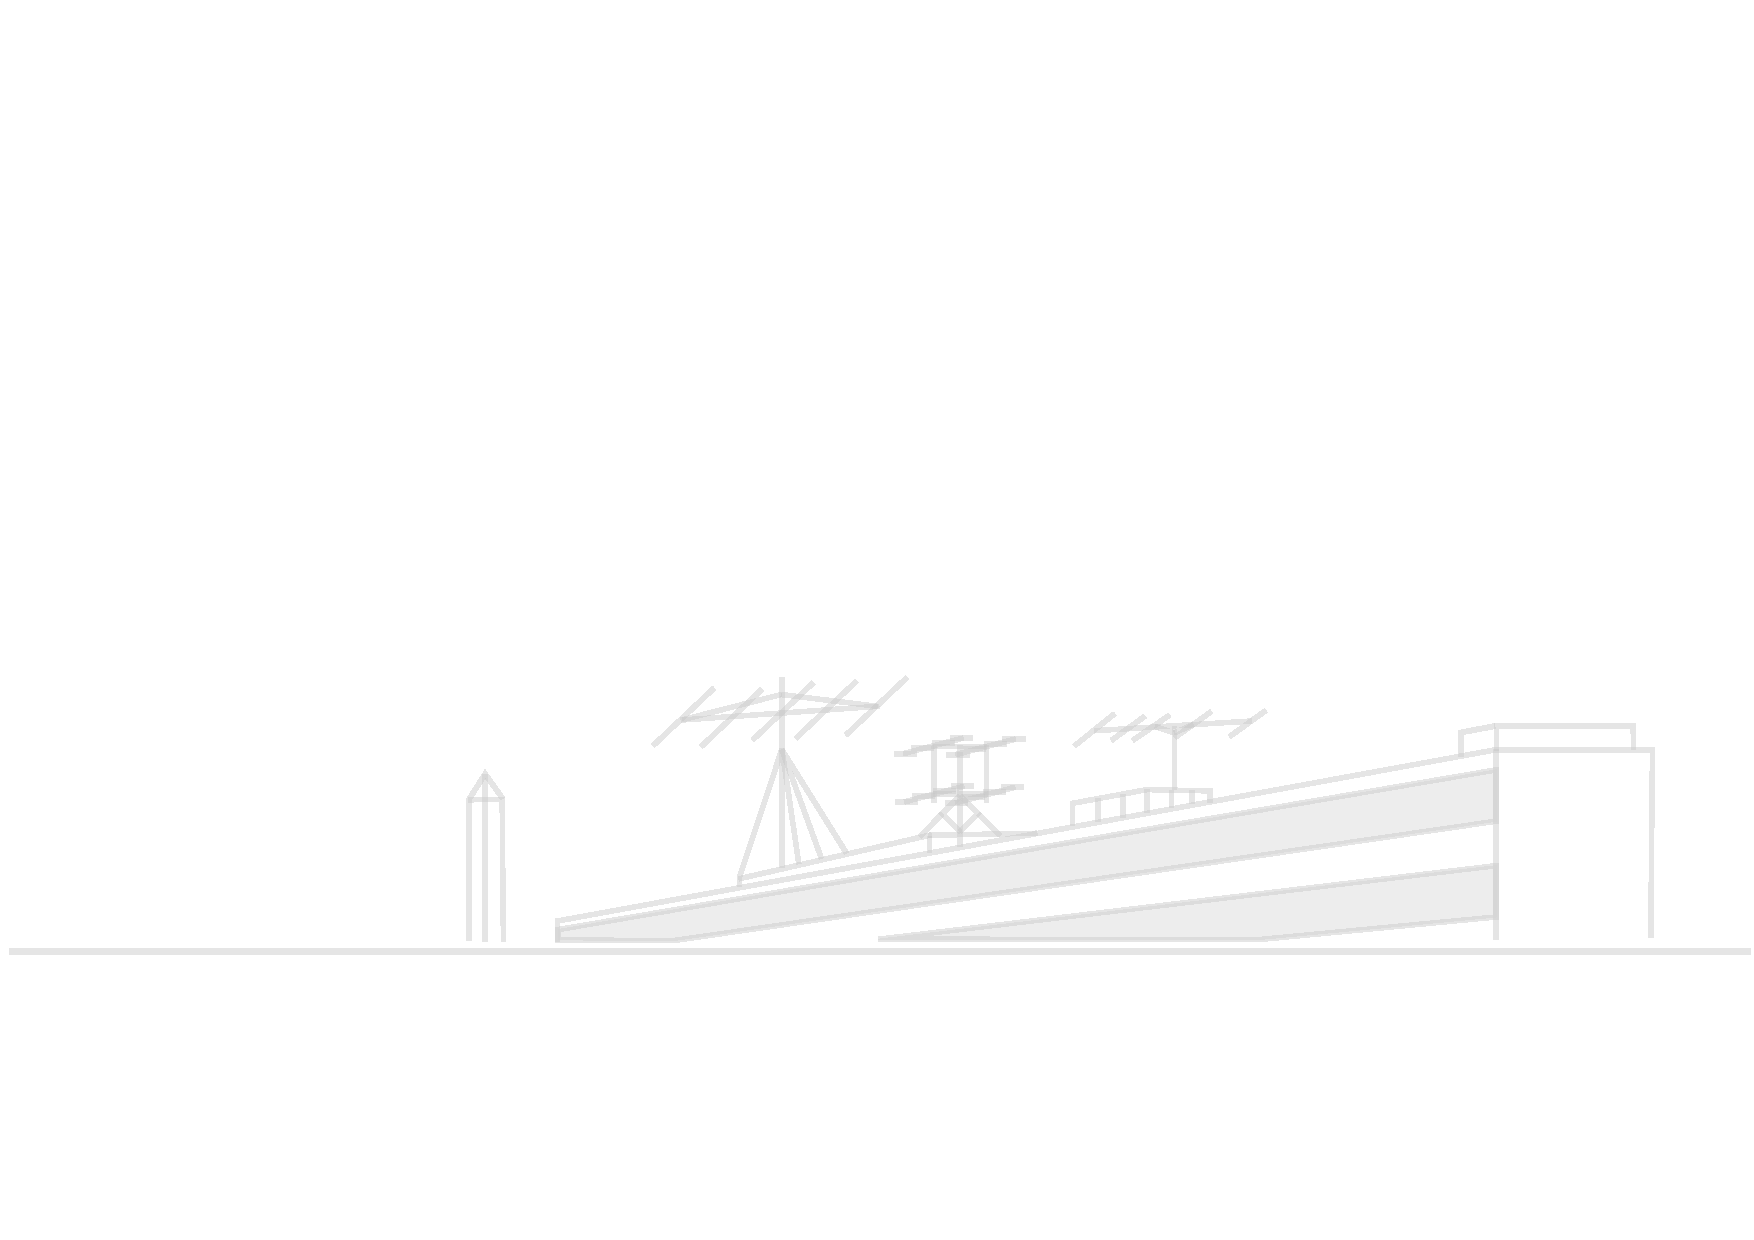
\includegraphics[width=17.8cm]{texdata/dk0tu_rooftop_background.pdf}
}

% Foliennummer einfügen
\setbeamertemplate{footline}[frame number]
%\setbeamertemplate{footline}{}

% Ändere das Zeichen vor jedem item
%\setbeamertemplate{itemize item}{\color{craneorange}$\blacktriangleright$}
%\setbeamertemplate{itemize subitem}{\color{craneorange}$\triangleright$}
%\setbeamertemplate{itemize subsubitem}{\color{craneorange}$\blacktriangleright$}

% Ändert die Blöcke 
\setbeamertemplate{blocks}[rounded][shadow=true]
% default | rounded [shadow=true|false]

%
% Eigene Kommandos
%

% Hack to get natbib and beamer working together. "The beamer user guide suggests
% that only the manual bibliography entry approach is supported"
% on some system it works out of the box, sometimes you need the hack :-(
% so check it --dl7bst
\ifdefined\newblock
    \relax
\else
    \newcommand{\newblock}{}
\fi

% \includedia command to generate png out of a dia file
% NEEDS installed dia and pdflatex option --shell-escape
\newcommand{\includedia}[1]{
    \immediate\write18{/usr/bin/dia #1.dia -e #1_diatmp.png -t png}
}

% RICHIG GROSSER FONT!
\newfont{\bigfont}{cmr10 at 144pt}
\newfont{\smallfont}{cmr10 at 8pt}

% Römische Ziffern
\makeatletter
\newcommand{\rmnum}[1]{\romannumeral #1}
\newcommand{\Rmnum}[1]{\expandafter\@slowromancap\romannumeral #1@}
\makeatother

% Schwarze Überschrift
%\setbeamercolor{frametitle}{fg=black}
%\setbeamercolor{title}{fg=black}

% Item- und Box-Farben
\definecolor{deepBlue}{HTML}{000066}
\setbeamercolor{itemize item}{fg=deepBlue}
\setbeamercolor{itemize subitem}{fg=deepBlue}
\setbeamercolor{description item}{fg=deepBlue}
\setbeamercolor{block title}{fg=deepBlue!100, bg=blue!15}
\setbeamercolor{block body}{fg=black, bg=blue!5}
\setbeamercolor{block title alerted}{fg=deepBlue, bg=red!75}
\setbeamercolor{block body alerted}{fg=black, bg=red!15}
\setbeamercolor*{block title example}{fg=blue!50, bg=blue!10}
\setbeamercolor*{block body example}{fg= blue, bg=blue!5}

%\setbeamercolor{section in head/foot}{parent=palette primary}
%\setbeamercolor{subsection in head/foot}{parent=palette secondary}
%\setbeamercolor{sidebar}{fg=darkblue,bg=yellow!90!orange}
%\setbeamercolor{title in sidebar}{fg=darkblue}
%\setbeamercolor{author in sidebar}{fg=darkblue}
%\setbeamercolor{section in sidebar}{fg=darkblue!10!black}
%\setbeamercolor{subsection in sidebar}{fg=darkblue!50!black}

% Titlepage Infos
\title{AFu-Kurs nach DJ4UF}
\author[DKØTU]{DKØTU\\ \footnotesize{Amateurfunkgruppe der TU Berlin}}
\institute[DKØTU]{\url{http://www.dk0tu.de} }

% PDF-Eigenschaften
\subject{DK0TU-Amateurfunkkurs nach DJ4UF}
\keywords{Amateurfunk Kurs HAM Radio Course CC-BY-NC-SA OpenSource TU Berlin DK0TU}

\subtitle{Betriebstechnik/Vorschriften 13: \\
RST-System, UTC, Logbuch, QSL-Karte \\[2em]}
\date{Stand 18.09.2017}
 \begin{document}

\begin{frame}
    \titlepage
    \vfill
    \begin{center}
        \ccbyncsaeu\\
        {\tiny This work is licensed under the \em{Creative Commons Attribution-NonCommercial-ShareAlike 3.0 License}.}\\[0.5ex]
         \tiny Amateurfunkgruppe der Technische Universität Berlin (AfuTUB), DKØTU
         %\includegraphics[scale=0.5]{img/DK0TU_Logo.pdf}
    \end{center}
\end{frame}


\section{Einleitung}

\begin{frame}
  \frametitle{Einleitung}

  Für den eigentlichen Spaß des Funkbetriebes braucht es etwas ``back
  office'':

  \begin{itemize}
    \item Logbuchführung
    \item QSL-Karten
  \end{itemize}

  \vspace{1cm}

  Benötigt: \emph{RST}-System und Umgang mit \emph{UTC}.

\end{frame}

\section{RST-System}

\begin{frame}
  \frametitle{RST-System}

  \textbf{R}eadability, Signal \textbf{S}trength, \textbf{T}one

  \begin{center}
    \begin{figure}
      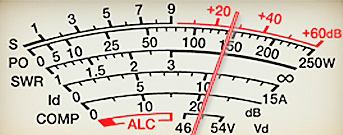
\includegraphics[width=0.8\textwidth,height=.45\textheight,keepaspectratio]{e10/S-Meter.jpg}
      \attribcaption{S-Meter}{Cqdx}{https://commons.wikimedia.org/wiki/File:S-Meter.jpg}{\ccbysa}
    \end{figure}
  \end{center}

  \begin{itemize}
    \item Zweck: Empfangsbeurteilung
    \item \emph{T} nur in Telegrafie
    \item Verwendung seit 1930er
  \end{itemize}

\end{frame}

\begin{frame}
  \frametitle{RST-System / Tabelle}

  \begin{center}
    \footnotesize
    \begin{tabular}{|l|l|l|l|}\hline
      & \textbf{R}eadability        & \textbf{S}trength & \textbf{T}one \\ \hline \hline
      1 & nicht lesbar                & $-48 dB$          & äußerst roh   \\ \hline
      2 & zeitweise lesbar            & $-42 dB$          & sehr roh      \\ \hline
      3 & mit Schwierigkeiten lesbar  & $-36 dB$          & roh           \\ \hline
      4 & ohne Schwierigkeiten lesbar & $-30 dB$          & leicht roh    \\ \hline
      5 & einwandfrei lesbar          & $-24 dB$          & musikalisch   \\ \hline
      6 &                             & $-18 dB$          & moduliert     \\ \hline
      7 &                             & $-12 dB$          & instabil      \\ \hline
      8 &                             & $-6 dB$           & etwas Brumm   \\ \hline
      9 &                             & $0dB$             & rein          \\ \hline
      9+x &                           & $+x dB$ über S9   &               \\ \hline
    \end{tabular}
  \end{center}

  S-Stufe 9 als Referenzspannung am $50 \Omega$-Antenneneingang:
  \begin{itemize}
    \item KW: $50\mu V$
    \item UKW: $5\mu V$
  \end{itemize}

\end{frame}

\begin{frame}
  \frametitle{RST-System / Abgeleitete Systeme}

  \begin{itemize}
    \item R: Sprechfunk (Relais)
    \item RS: Sprechfunk (p2p)
    \item RSV: \textbf{V}ideo - SSTV/ATV
    \item RSQ: \textbf{Q}uality - digitalen Betriebsarten
    \item RSA: \textbf{A}urora - Tonrapport wäre quatsch $\rightarrow$ ``A'' geben
  \end{itemize}

\end{frame}

\begin{frame}
  \frametitle{RST-System / S-Stufe}

  Bedenke: Eine S-Stufe = $6 dB$

  \begin{itemize}
    \item gemessen an Spannung (Feldgröße) $\rightarrow$ Verdopplung
    \item Leistungsgröße $\rightarrow$ Vervierfachung!
  \end{itemize}

  \vspace{1cm}

  Beispiel\footnote{Prüfungskatalog Frage BB303}:

  \begin{exampleblock}{Um wie viel S-Stufen müsste die S-Meter-Anzeige Ihres
    Empfängers steigen, wenn Ihr Partner die Sendeleistung von 100
    Watt auf 400 Watt erhöht?}
    \only<1>{\vspace{1pc}}\only<2>{$\rightarrow$ Um eine S-Stufe}
  \end{exampleblock}

\end{frame}

\begin{frame}
  \frametitle{RST-System / S-Stufe}

  Noch ein Beispiel\footnote{Prüfungskatalog Frage BB307}:

  \begin{exampleblock}{Durch ``Fading'' sinkt die S-Meter-Anzeige von S9 auf S8. Auf
    welchen Wert sinkt dabei die Empfänger-Eingangsspannung ab,
    wenn bei S9 am Empfängereingang $50\mu V$ anliegen? Die
    Empfänger-Eingangsspannung sinkt auf}
    \only<1>{\vspace{1pc}}\only<2>{$\rightarrow 25\mu V$}
  \end{exampleblock}

\end{frame}

\section{UTC}

\begin{frame}
  \frametitle{\textbf{U}niversal \textbf{T}ime, \textbf{C}oordinated}

  \begin{center}
    \begin{figure}
      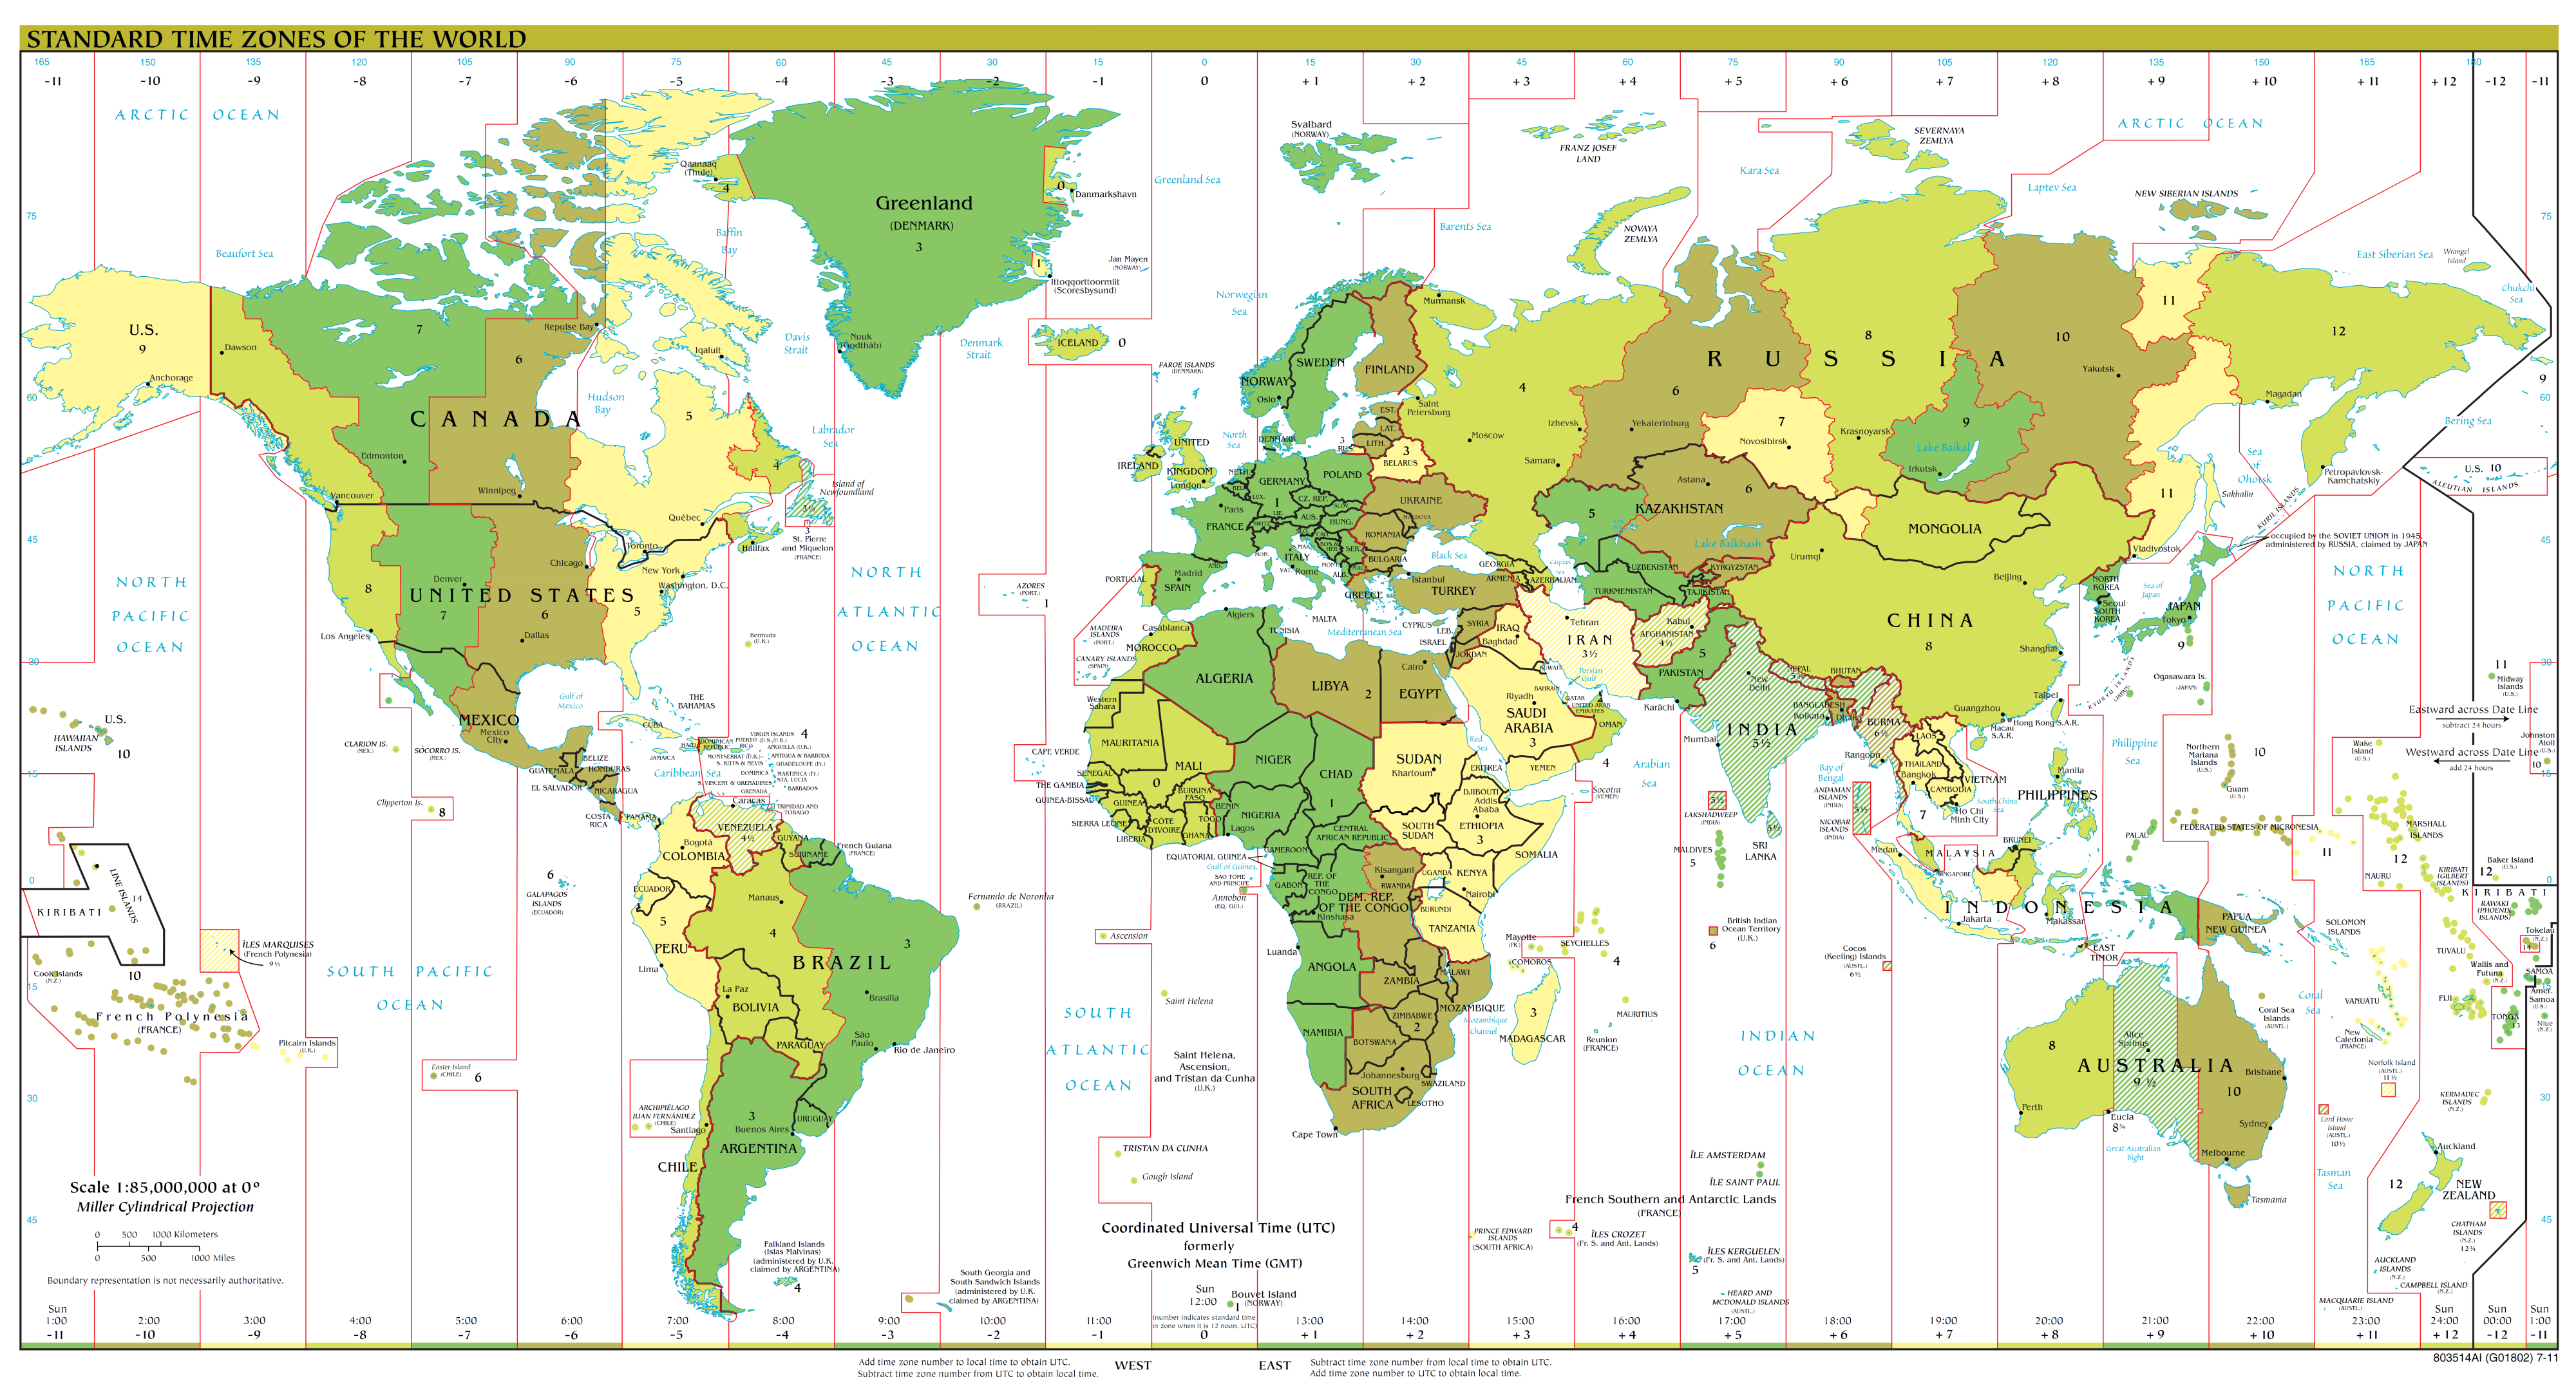
\includegraphics[width=0.7\textwidth,height=.55\textheight,keepaspectratio]{bv13/Standard_time_zones_of_the_world.png}
      \attribcaption{Zeitzonen der Welt seit dem 20.09.2011}{TimeZonesBoy}{https://commons.wikimedia.org/wiki/File:Standard_time_zones_of_the_world.png}{\ccbysa}
    \end{figure}
  \end{center}

  Bezugsachse: lokale ``Sonnenzeit'' am Nullmeridian durch
    London-Greenwich\footnote{früher übliche Bezeichnung
    \emph{Greenwich Mean Time (GMT)}}

\end{frame}

\begin{frame}
  \frametitle{UTC}

  \begin{center}
    \begin{figure}
      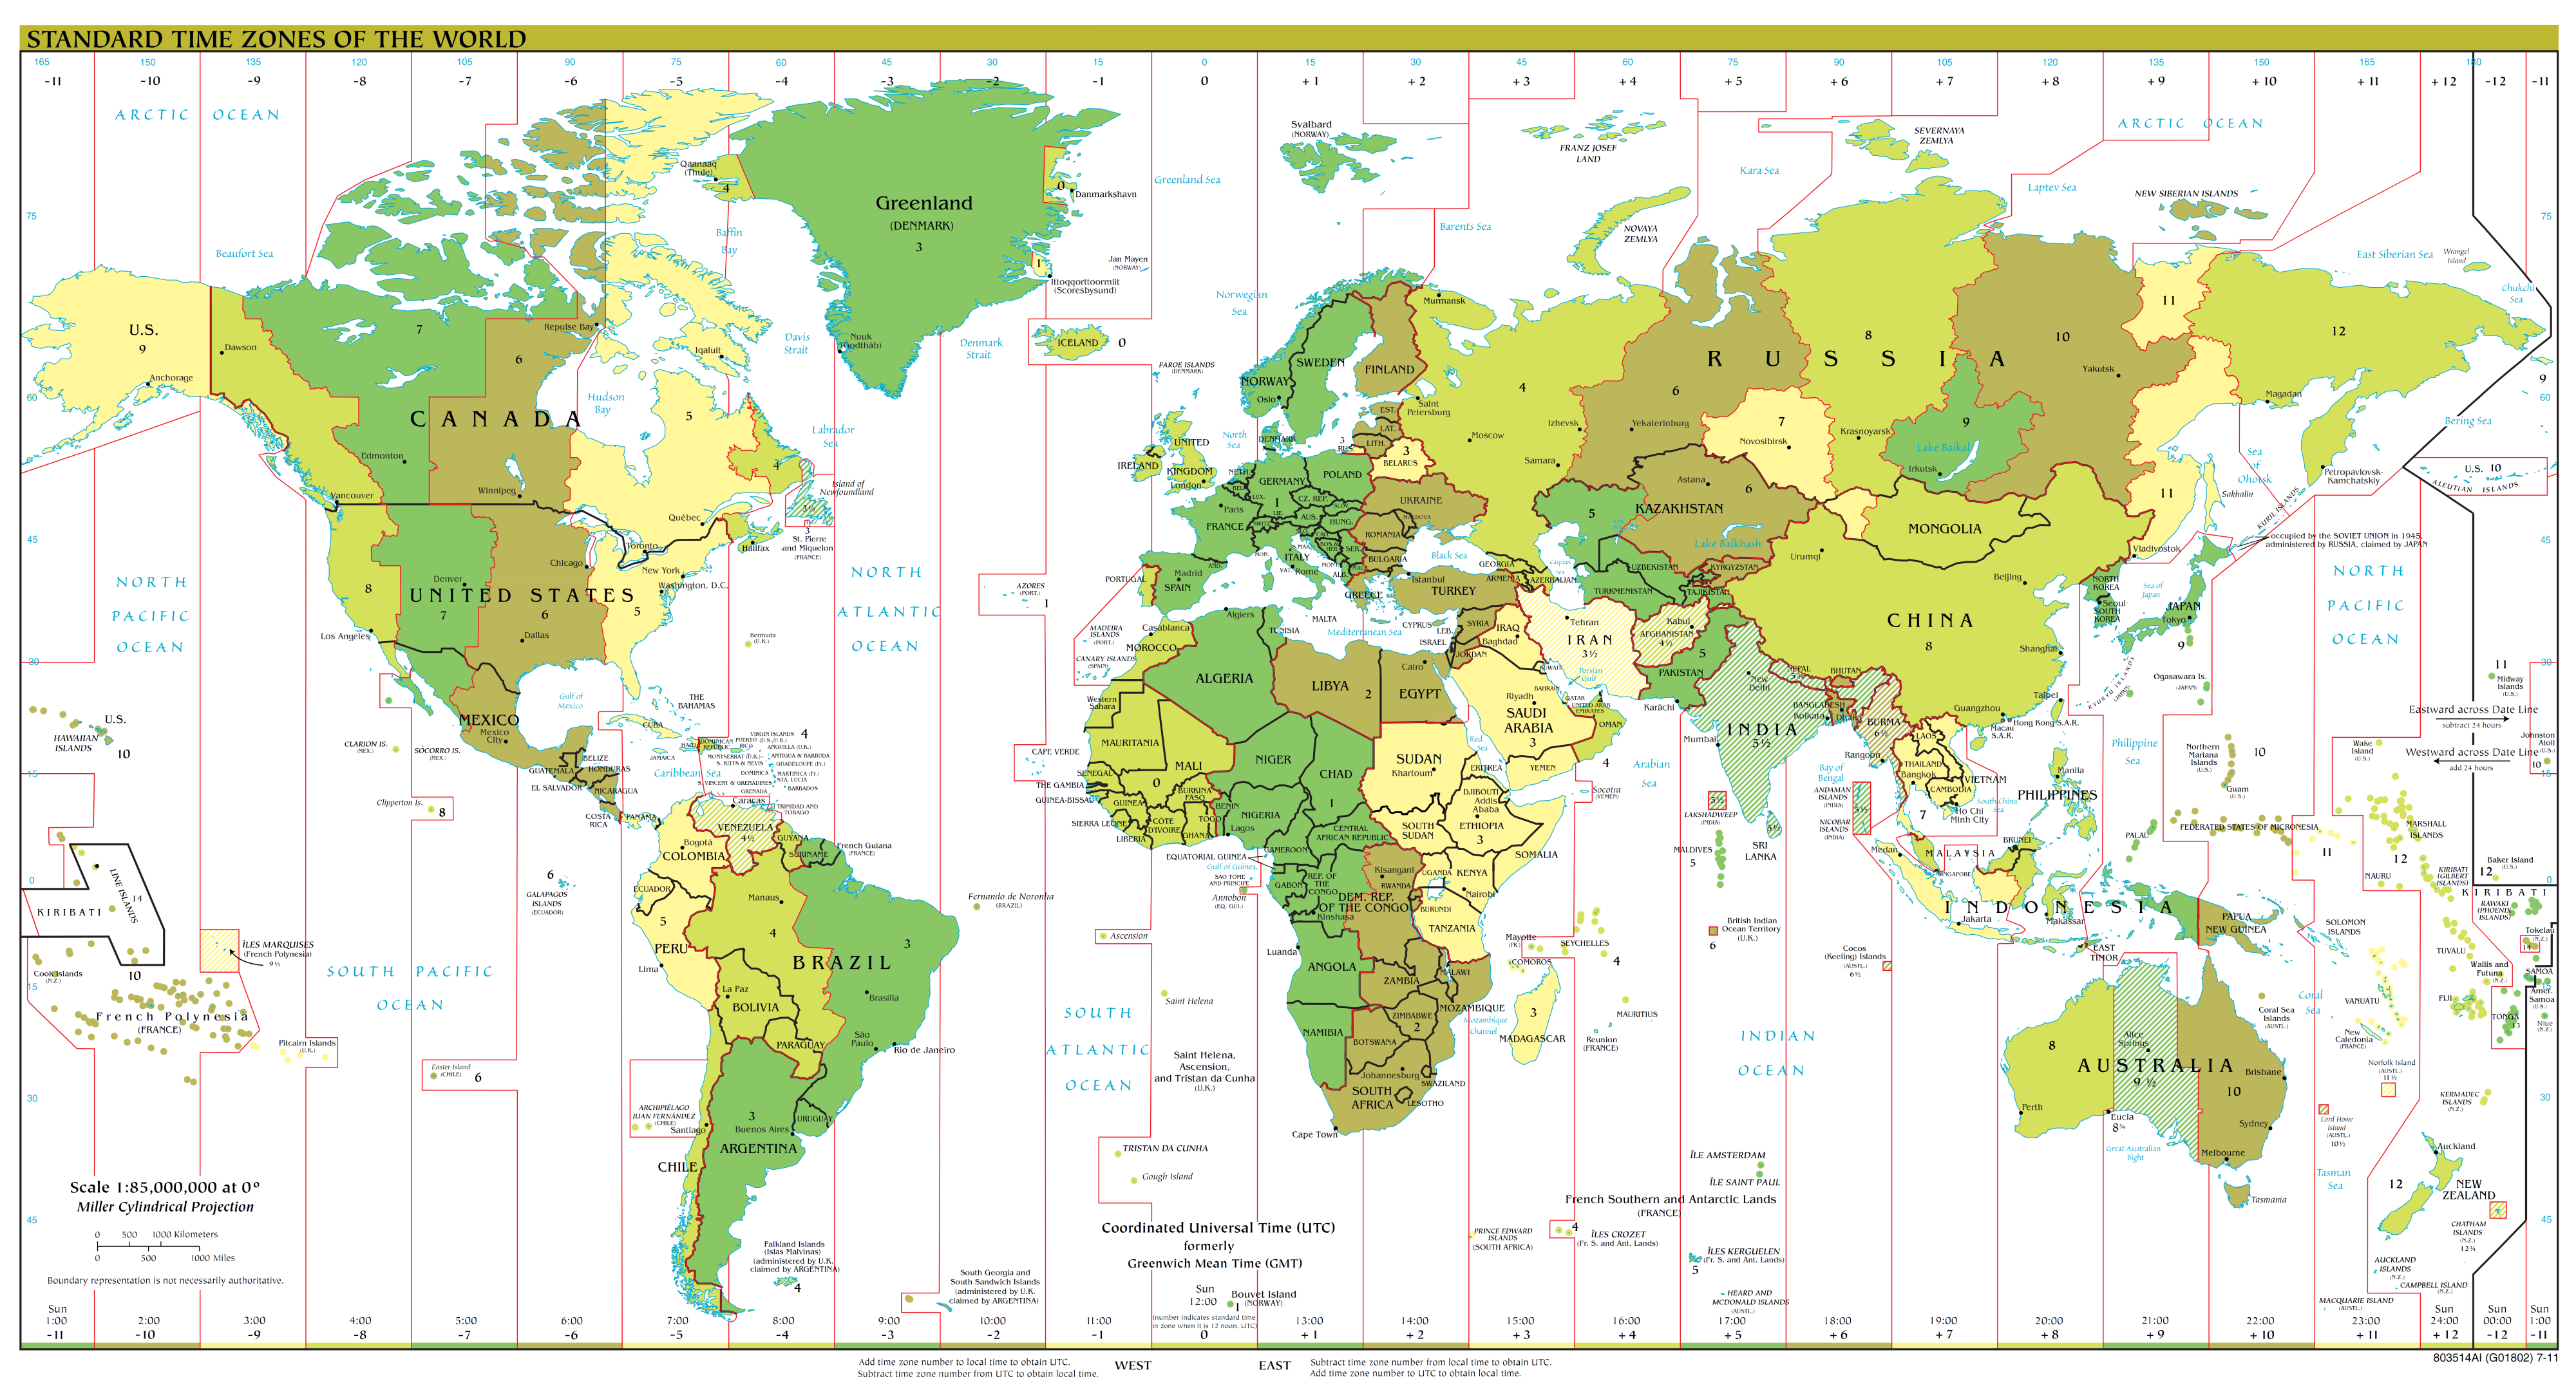
\includegraphics[width=0.5\textwidth,height=.35\textheight,keepaspectratio]{bv13/Standard_time_zones_of_the_world.png}
      \attribcaption{Zeitzonen der Welt seit dem 20.09.2011}{TimeZonesBoy}{https://commons.wikimedia.org/wiki/File:Standard_time_zones_of_the_world.png}{\ccbysa}
    \end{figure}
  \end{center}

  \begin{itemize}
    \item weit mehr als 24 Zeitzonen: UTC-12 bis UTC+14 (Kartenzoom lohnt sich)
      - nicht immer volle Stunden
    \item Deutschland:
      \begin{itemize}
        \item UTC+1 = CET/MEZ
        \item UTC+2 = CEST/MESZ
      \end{itemize}
  \end{itemize}

  Da AFu international $\rightarrow$ alleinige Verwendung von UTC!

\end{frame}

\section{Logbook}

\begin{frame}
  \frametitle{Logbook}

  ``Stationstagebuch, das ein Funkamateur freiwillig führt oder in besonderen
  Fällen führen muss.''

  %todo aktuelles Papierlogbild?
  \begin{center}
    \begin{figure}
      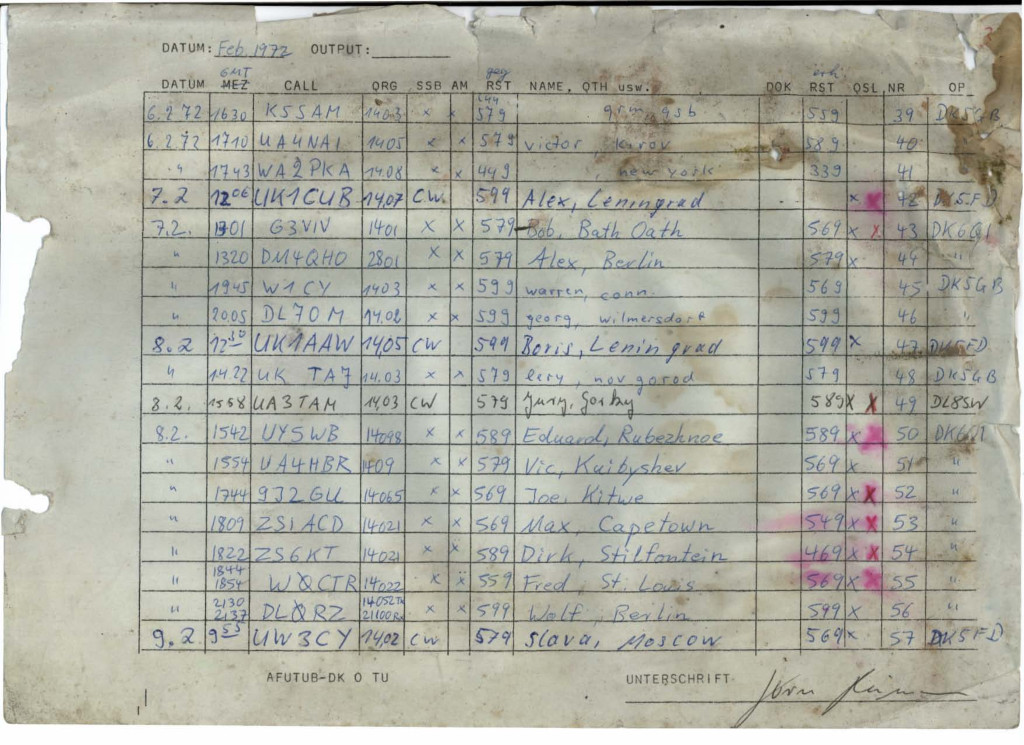
\includegraphics[width=0.55\textwidth,height=.7\textheight,keepaspectratio]{bv13/DK0TU_LOG_KW_1972-02_Auszug.jpg}
      \caption{DKØTU Kurzwellenlog Feb. 1972 (Auszug, nach Wasserschaden)}
    \end{figure}
  \end{center}

\end{frame}

\begin{frame}
  \frametitle{Logbook}

  \begin{columns}
    \column{.4\textwidth}
    \begin{center}
      \begin{figure}
        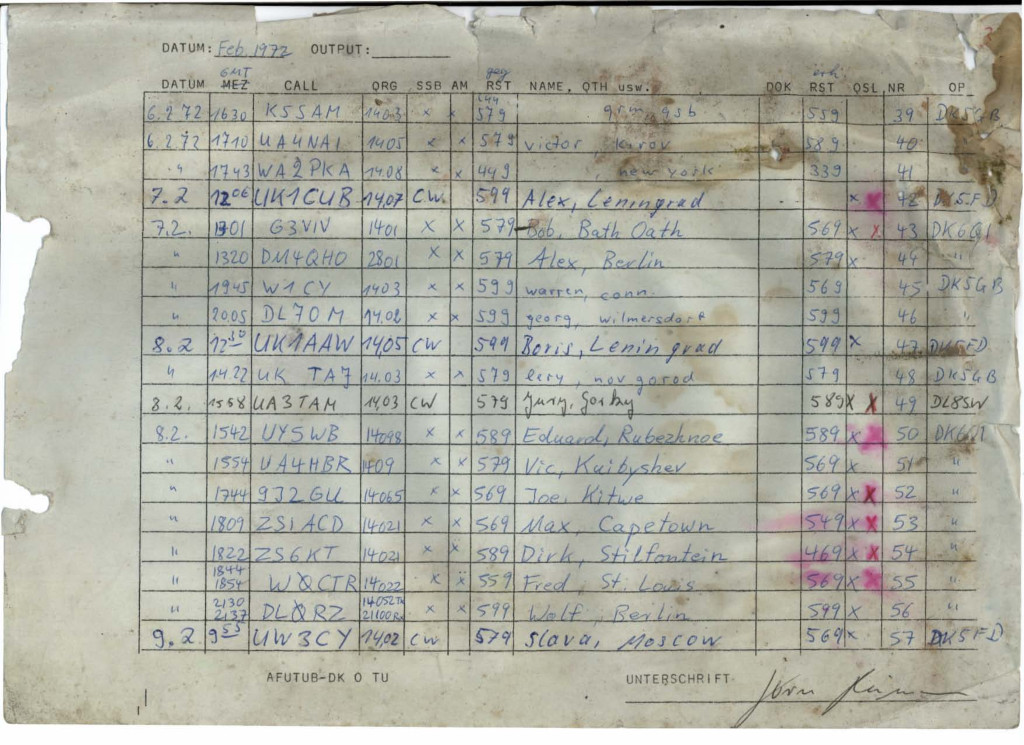
\includegraphics[width=\textwidth,height=.8\textheight,keepaspectratio]{bv13/DK0TU_LOG_KW_1972-02_Auszug.jpg}
        \caption{DKØTU Kurzwellenlog Feb. 1972 (Auszug, nach Wasserschaden)}
      \end{figure}
    \end{center}

  \column{.6\textwidth}
    Je Aussendung:

    \begin{itemize}
      \item Tag, Uhrzeit (immer UTC!)
      \item Frequenz
      \item Rufzeichen
      \item Rapporte
      \item ggf. Aufzeichnungen über Bedingungen, Sendeleistung, Antenne, ...
    \end{itemize}

    Praktisch für sich selbst oder auch einen \emph{EMV}-Fall.
  \end{columns}

\end{frame}

\subsection{Digitallog}

\begin{frame}
  \frametitle{Logbook / Digitallog}

  Papierlog oder Computerlog: Minimalistisch vs. einfache Handhabung und
  Katalogisierung:

  \begin{center}
    \begin{figure}
      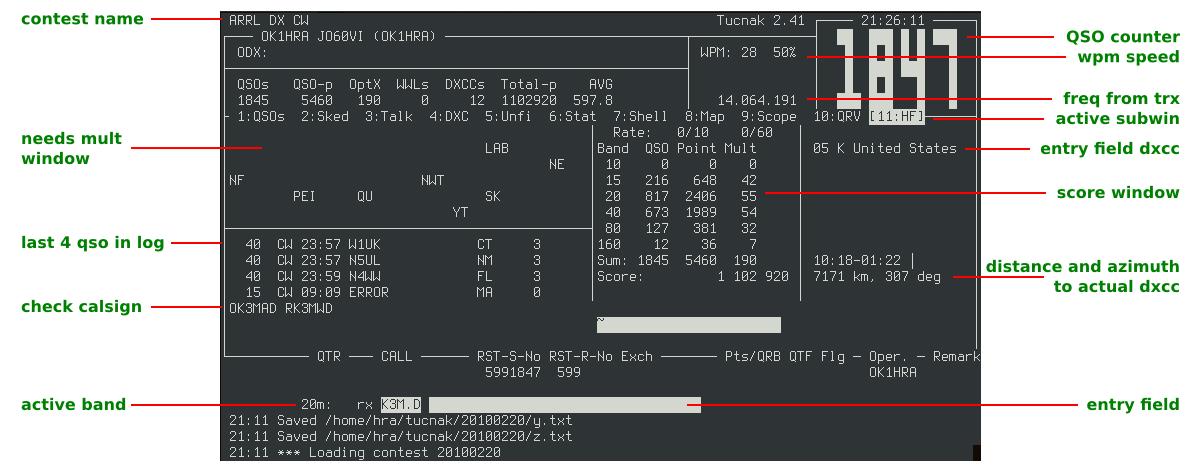
\includegraphics[width=1\textwidth,height=.75\textheight,keepaspectratio]{bv13/tucnak_Hf-10.png}
      \caption{Tucnak Contest-Log \hyperlink{refs}{\cite{tucn}}}
    \end{figure}
  \end{center}

\end{frame}

\begin{frame}
  \frametitle{Logbook / Digitallog}
  \begin{center}
    \begin{figure}
      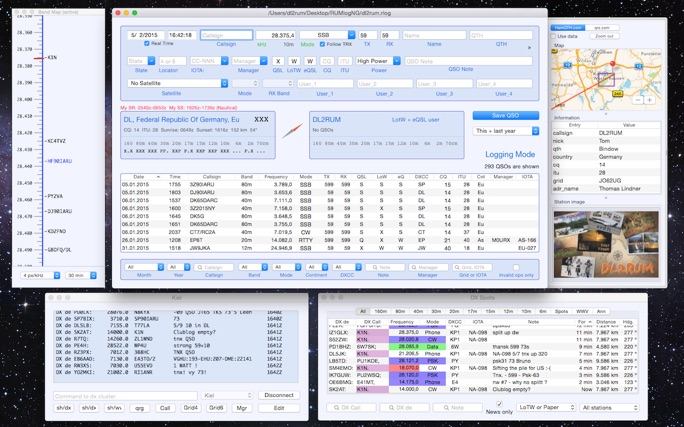
\includegraphics[width=\textwidth,height=.75\textheight,keepaspectratio]{bv13/rumlogng.jpg}
      \caption{Aktuelle MacOS Applikation RUMlogNG \hyperlink{refs}{\cite{rumlog}}}
    \end{figure}
  \end{center}
\end{frame}

\begin{frame}
  \frametitle{Logbook / Digitallog}

  \begin{columns}
    \column{.45\textwidth}
    \begin{center}
      \begin{figure}
        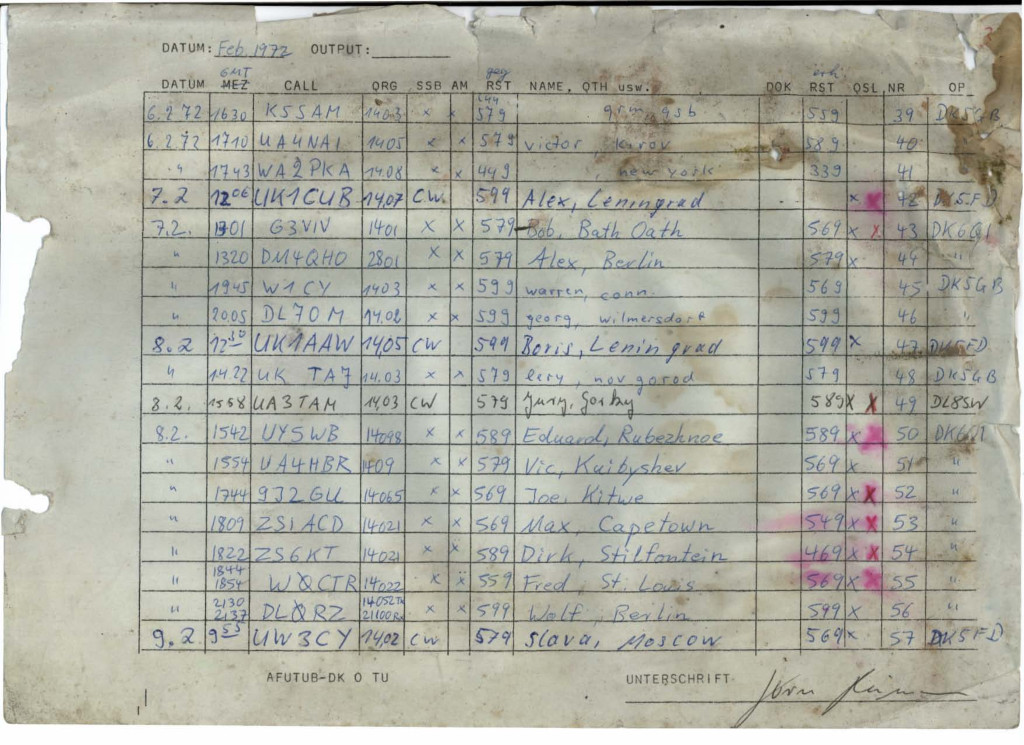
\includegraphics[height=0.25\textheight,width=\textwidth,keepaspectratio]{bv13/DK0TU_LOG_KW_1972-02_Auszug.jpg}
        \caption{DKØTU Kurzwellenlog Feb. 1972}
      \end{figure}
    \end{center}
    \column{.1\textwidth}
    \hspace{2pc}$\rightarrow$\hspace{1pc}
    \column{.45\textwidth}
    \begin{center}
      \begin{figure}
        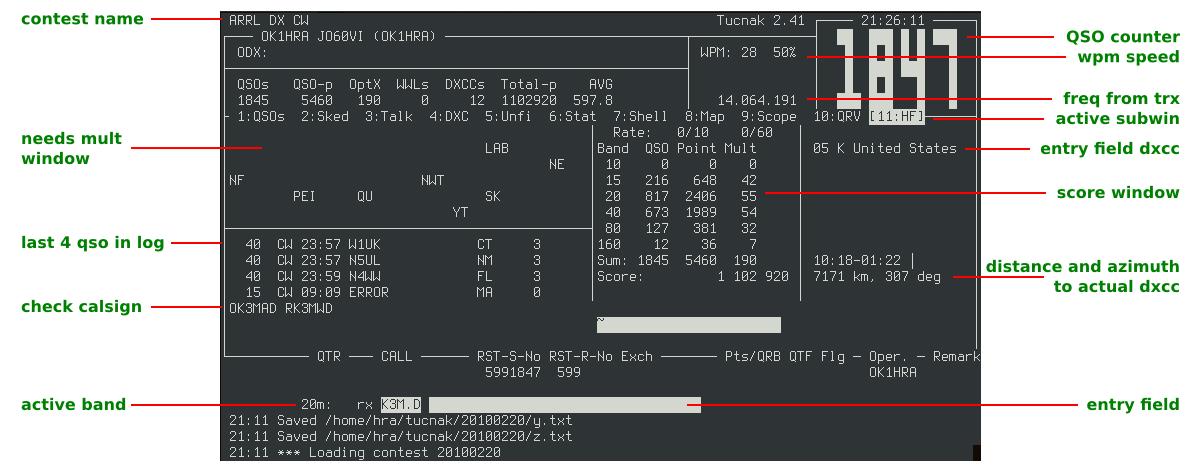
\includegraphics[height=0.25\textheight,width=\textwidth,keepaspectratio]{bv13/tucnak_Hf-10.png}
        \caption{Tucknak Contest-Log}
      \end{figure}
    \end{center}
  \end{columns}

  \begin{center}
    \begin{itemize}
      \item Uhrzeit automatisch
      \item QRG vom TRX übertragen
      \item QTF\footnote{Antennenrichtung}-Anzeige oder -Steuerung
      \item Call-Datenbanken
      \item DX-Cluster
      \item Sync im LAN/WAN für Multi-Op
      \item je nach Logprogramm weitere Optionen
    \end{itemize}
  \end{center}

\end{frame}

\subsection{Beispiele}

\begin{frame}
  \frametitle{Beispiel: Papierlog}

  \begin{center}
    \begin{figure}
      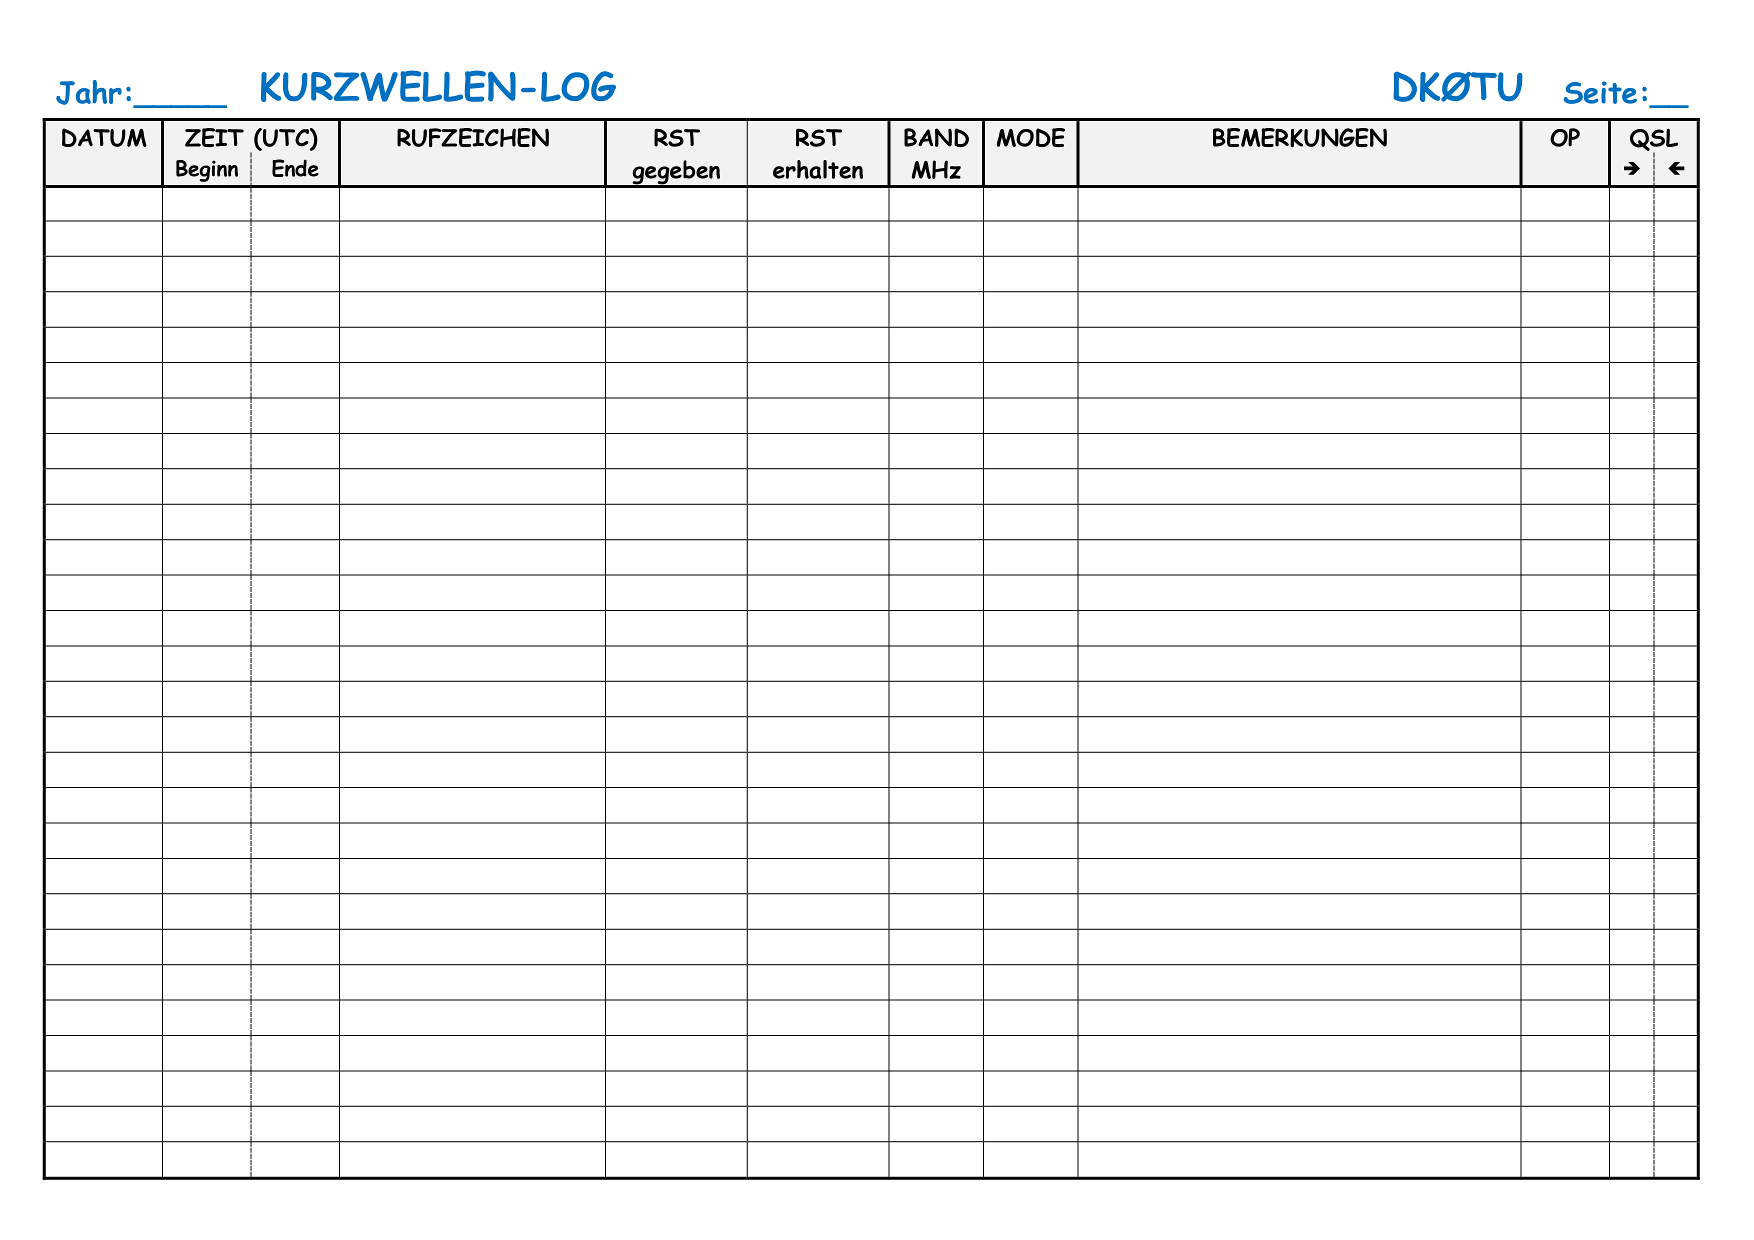
\includegraphics[height=.75\textheight]{bv13/dk0tu_log_kw.png}
      \caption{Kurzwellenlogbuch bei DKØTU}
    \end{figure}
  \end{center}

\end{frame}

\begin{frame}
  \frametitle{Beispiele: Software}

  \begin{center}

    \Large Demo... \\[3em]

    \normalsize $\Rightarrow$ Export: \ExternalLink\url{http://www.dk0tu.de/Logbook}

  \end{center}

\end{frame}

\subsection{Angeordnete Logbuchführung}

\begin{frame}
  \frametitle{Logbuchführung / Angeordnete Logbuchführung}

  Heutzutage ist die Logbuchführung freiwillig -- im Falle einer Störung nicht.
  Die ``zuständige Behörde'' (\emph{BNetzA}) kann das anordnen.

  \begin{center}
    \begin{figure}
      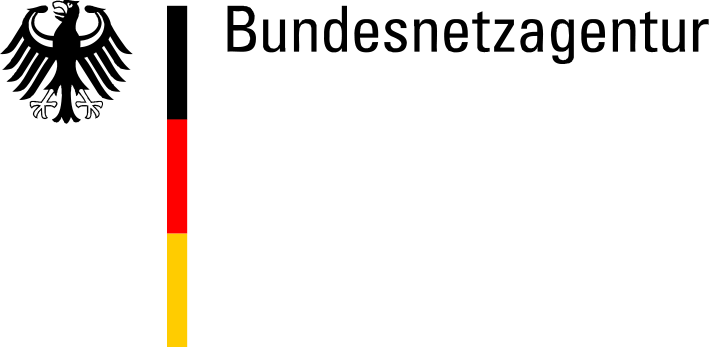
\includegraphics[width=0.3\textwidth,height=.3\textheight,keepaspectratio]{bv13/Bundesnetzagentur_logo_709px.png}
      \attribcaption{Bundesnetzagentur}{Bundesnetzagentur}{https://de.wikipedia.org/wiki/Datei:Bundesnetzagentur_logo.svg}{\ccpd}
    \end{figure}
  \end{center}

  \begin{itemize}
    \item Log muss angeordnete Zeit aufgehoben werden
    \item digitales Log zulässig
    \item bei Softwarewechsel muss die alte verfügbar bleiben
    \item Export in maschinenlesbares Logbuchformat
  \end{itemize}

\end{frame}

\begin{frame}
  \frametitle{Logbuchführung / Angeordnete Logbuchführung}

  \begin{exampleblock}{Ausbildungsfunkbetrieb}
    AfuV §12
    \begin{quote}
      (4) Beim Ausbildungsfunkbetrieb sind von dem Auszubildenden Angaben über den Funkbetrieb schriftlich festzuhalten und vom Ausbilder zu bestätigen. Dieser hat die Aufzeichnungen ein Jahr aufzubewahren.
    \end{quote}
  \end{exampleblock}
\end{frame}


\section{QSL-Karte}

\begin{frame}
  \frametitle{QSL-Karte}

  \emph{QSL} - wir erinnern uns aus \texttt{BV03} - Empfangsbestätigung \\[1em]

  \begin{center}
    \begin{figure}
      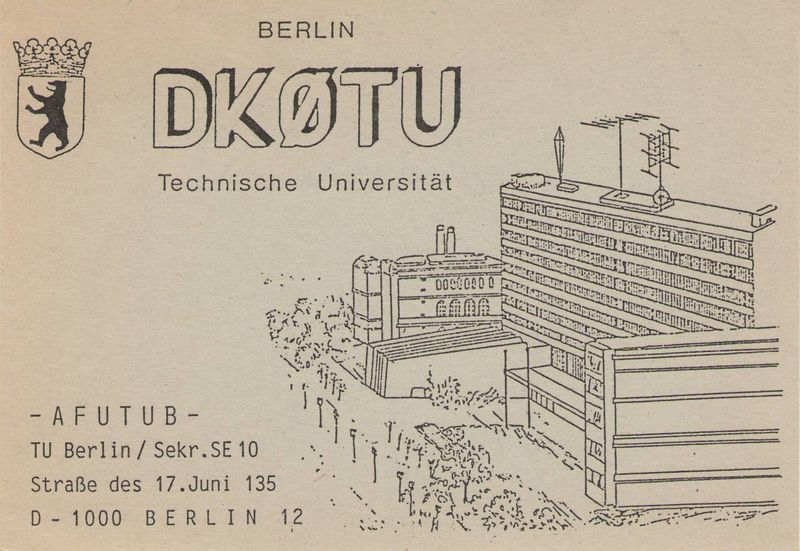
\includegraphics[width=0.6\textwidth,height=.6\textheight,keepaspectratio]{bv13/DK0TU_1.jpg}
      \caption{Historische QSL-Karte}
    \end{figure}
  \end{center}

  $\rightarrow$ traditionell auch mit einer ``Ansichtskarte'' bei KW oder UKW-DX

\end{frame}

\begin{frame}
  \frametitle{QSL-Karte}

  \begin{center}
    \begin{figure}
      
\includegraphics[width=0.5\textwidth,height=.5\textheight,keepaspectratio]{bv13/DK0TU_0.jpg}
      \caption{Historische QSL-Karte}
    \end{figure}
  \end{center}

  \begin{itemize}
    \item für SWL lange Zeit einziger Rückkanal
    \item schriftl. Bestätigung der Angaben
    %\item Beantragung Amateurfunk-Diplome
    \item individuell sehr verschieden gestaltet
  \end{itemize}

\end{frame}

\begin{frame}
  \frametitle{QSL-Karte / Informationen}

  \begin{exampleblock}{Welche Angaben sollten mind. enthalten sein?}
    \only<1>{$\rightarrow$ Tafel}
    \only<2>{
    Im Prinzip Daten aus dem \textbf{Logbook}:
    \begin{itemize}
      \item Rufzeichen
      \item Rufzeichen der Gegenstation
      \item Datum
      \item Uhrzeit (UTC)
      \item Frequenz
      \item Betriebsart
      \item Signal-Rapport
      \item Unterschrift des Op
    \end{itemize}
    }
  \end{exampleblock}

  \only<2>{
  \footnotesize{Besonderheit\footnote{z.B. bei \emph{DXpeditionen}}:
  \emph{``QSL via [Call]''} $\rightarrow$ QSL-Manager}
  }

\end{frame}

\begin{frame}
  \frametitle{QSL-Karte / Informationen}

  \begin{center}
    \begin{figure}
      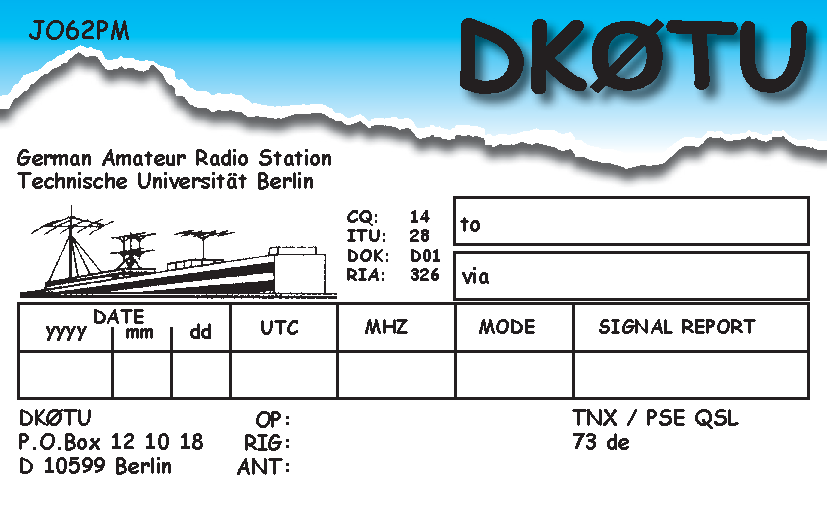
\includegraphics[width=0.9\textwidth,height=.75\textheight,keepaspectratio]{bv13/dk0tu_qsl2.pdf}
      \caption{Aktuelle QSL-Karte}
    \end{figure}
  \end{center}

\end{frame}

\begin{frame}
  \frametitle{QSL-Karte / Versand}

  \begin{itemize}
    \item kostenfrei \emph{``via bureau''}
    \item direkte Zusendung durch Adresse aus \emph{int. Callbook} oder Internet
  \end{itemize}

  Für besonders Eilige oder Länder ohne Radio Clubs: Mit Versand der Karte
  Antwortbriefumschlag (\emph{SAE}\footnote{Self-Addressed Envelope}) und
  \emph{IRC}\footnote{International Reply Coupon}s zwei 1\$-Noten beilegen. \\[2em]

  \pause

  Noch eiliger: Online-QSL-Karten
  \begin{itemize}
    \item eQSL \ExternalLink\url{https://www.eqsl.cc/}
    \item LoTW \ExternalLink\url{https://lotw.arrl.org/}
  \end{itemize}

\end{frame}

\subsection{eQSL}

\begin{frame}
  \frametitle{QSL-Karte / eQSL}

  im Prinzip wie \textbf{e}Mail

  \begin{center}
    \begin{figure}
      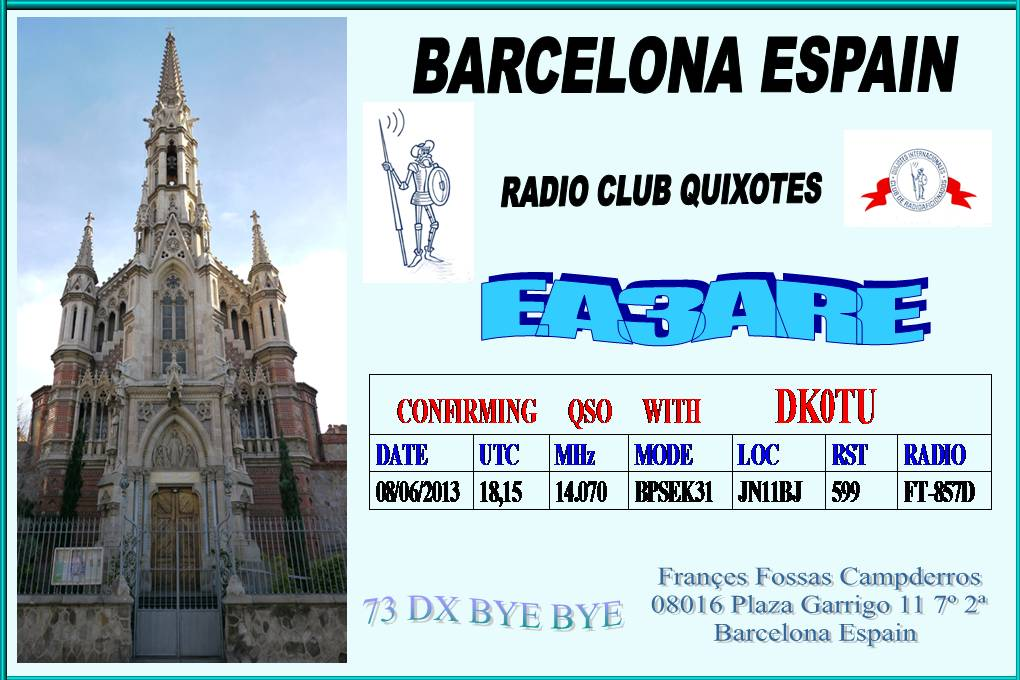
\includegraphics[width=0.4\textwidth,height=.4\textheight,keepaspectratio]{bv13/eQSL_DK0TU-EA3ARE.jpg}
      \caption{Empfangene eQSL-Karte}
    \end{figure}
  \end{center}

  \begin{itemize}
    \item minimaler Kostenaufwand
    \item Ausdruck nur bei Bedarf
    \item weniger ``Flair''
  \end{itemize}

  Wie bei E-Mail gibt es diverse Webdienste oder Programme.

\end{frame}

\subsection{SSTV}

\begin{frame}
  \frametitle{QSL-Karte / SSTV}

  Keine QSL-Karte, aber manchmal wird einfach das empfangene SSTV-Bild zur
  Bestätigung per E-Mail zurückgesendet.

  \begin{center}
    \begin{figure}
      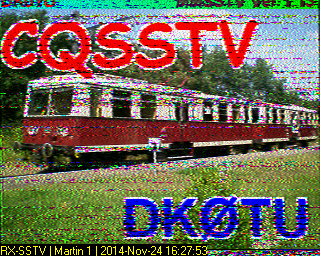
\includegraphics[width=0.6\textwidth,height=.6\textheight,keepaspectratio]{bv13/QSL_SSTV_2014-11-24_162753.png}
      \caption{Empfangenes SSTV-Bild}
    \end{figure}
  \end{center}

\end{frame}

\section{Sonderstationen}

\begin{frame}
  \frametitle{Sonderstationen}

  Einige HAMs sammeln besondere Stationen:

  \begin{center}
    \begin{figure}
      
\includegraphics[width=0.4\textwidth,height=.35\textheight,keepaspectratio]{bv13/DK0TU_SDOK_FSB13.jpg}
      \caption{Limitierte QSL-Karte von DKØTU mit Sonder-DOK FSB13}
    \end{figure}
  \end{center}

  \begin{itemize}
    \item Calls zu bestimmten Veranstaltungen, z.B.
      \emph{DKØIFA}\footnote{zur Internationale Funkausstellung (IFA)}
    \item Sonder-DOK\footnote{Distrikts-Ortsverbands-Kenner}s, z.B.
      \emph{FSB13}\footnote{zum Jubiläum der ehemaligen Field Station
      Berlin (Teufelsberg)}
  \end{itemize}

\end{frame}

\section{Diplome}

\begin{frame}
  \frametitle{Diplome}

  %todo Foto ARRL Diplom

  Auszeichnung\footnote{meist Urkundenpapier, aber auch diverse andere
  Gegenstände} für besondere Leistungen im Amateurfunk.

  Herausgeber z.B.

  \begin{itemize}
    \item Radioclubs
    \item Ortsverbände
    \item Länder
  \end{itemize}

\end{frame}

\begin{frame}
  \frametitle{Diplome / Beispiele}

  Bekannteste Diplome z.B.

  \begin{itemize}
    \item DXCC\footnote{DX century club}-Diplom für $>100$ Länder
    \item DLD\footnote{Deutschland Diplom} für $>100$ \emph{OV}s
    \item Berlin-Diplom\footnote{\ExternalLink\url{http://www.darc.de/distrikte/d/berlin-diplom/}}
    \item JO62-Diplom\footnote{\ExternalLink\url{http://www.ov-d20.de/diplom_jo62.htm}}
    \item ... ``All \$Achievement Award''
  \end{itemize}

  Beantragung vom Operator selbst. Nachweis: QSL-Karten, relevante
  Logbuchauszüge oder Bestätigung durch andere \emph{HAM}s.

\end{frame}

\renewcommand{\refname}{Referenzen}

\hypertarget{refs}{}
\textcolor{white}{} \\ %\vspace{} geht nicht
\Large Referenzen/Links
\footnotesize

\begin{thebibliography}{}

  \bibitem{dj4uf} Moltrecht B/V 13: \\
    \url{https://www.darc.de/der-club/referate/ajw/lehrgang-bv/bv13/}
  \bibitem{wp}    Wikipedia DE: \\
    \url{https://de.wikipedia.org/wiki/RST-System}\\
    \url{https://de.wikipedia.org/wiki/RSQ-System}\\
    \url{https://de.wikipedia.org/wiki/Koordinierte_Weltzeit}\\
    \url{https://de.wikipedia.org/wiki/Bundesnetzagentur}\\
  %\bibitem{we}    Wikipedia EN: \\
  \bibitem{tucn}  \url{http://tucnak.nagano.cz/wiki/File:Hf-10.png}\\
  \bibitem{rumlog} \url{http://www.dl2rum.de/rumsoft/RUMLog.html}\\
\end{thebibliography}

% Hier könnte noch eine Kontaktfolie stehen

\end{document}

